\documentclass[
    a4paper,
    12pt,
    addpoints,
    % answers
]{exam} % Documentação: https://ctan.dcc.uchile.cl/macros/latex/contrib/exam/examdoc.pdf
% -------------Início do preâmbulo-------------
\usepackage[utf8]{inputenc} 
\usepackage[T1]{fontenc}
\usepackage[lmargin=3cm,rmargin=2cm,tmargin=2cm,bmargin=2cm]{geometry} % Margens 
\usepackage[brazil]{babel} 
\usepackage{amssymb} % Símbolos (principalmente matemáticos)

\usepackage{graphicx} % Suporte ao \includegraphics[options]{name}
\usepackage{xcolor} % Cores
\usepackage[
    bookmarks=true,         % show bookmarks bar?
    unicode=false,          % non-Latin characters in Acrobat’s bookmarks
    pdftoolbar=true,        % show Acrobat’s toolbar?
    pdfmenubar=true,        % show Acrobat’s menu?
    pdffitwindow=false,     % window fit to page when opened
    pdfstartview={FitW},    % fits the width of the page to the window
    pdftitle={My title},    % title
    pdfauthor={Author},     % author
    pdfsubject={Subject},   % subject of the document
    pdfcreator={Creator},   % creator of the document
    pdfproducer={Producer}, % producer of the document
    pdfkeywords={keyword1, key2, key3}, % list of keywords
    pdfnewwindow=true,      % links in new PDF window
    colorlinks=true,       % false: boxed links; true: colored links
    linkcolor=black,          % color of internal links (change box color with linkbordercolor)
    citecolor=green,        % color of links to bibliography
    filecolor=cyan,         % color of file links
    urlcolor=magenta        % color of external links
]{hyperref} % Referência cruzada com direcionamento automático


% Os itens a seguir servem para editar os cabeçalhos e os rodapés.
% Eles são específicos para esta classe.

% Determina que as páginas terão cabeçalho e rodapé:
% \pagestyle{empty} % Sem cabeçalho sem rodapé
% \pagestyle{head} % Com cabeçalho sem rodapé
% \pagestyle{foot} % Sem cabeçalho com rodapé
\pagestyle{headandfoot} % Com cabeçalho com rodapé
\firstpageheadrule % Linha horizontal no cabeçalho na primeira página do documento
% Cabeçalho da primeira página:
% \firstpageheader{parte esqueda}{parte central}{parte direita} 
\firstpageheader{Nightwind \\ Professor}{\large \sffamily Primeiro Trabalho \\ Disciplina: \LaTeX}{25 de março de 2021}

\firstpagefootrule % Linha horizontal no rodapé na primeira página do documento
% \firstpagefooter{parte esqueda}{parte central}{parte direita} 
\firstpagefooter{\bfseries \sffamily Nightwind}{}{\itshape \ttfamily Bom Trabalho!}

\runningheadrule % Linha horizontal no cabeçalho nas demais páginas do documento
% \runningheader{parte esqueda}{parte central}{parte direita} 
\runningheader{Primeiro Trabalho}{}{\makebox[5cm]{Matrícula:\enspace\hrulefill}}
% \runningfooter{parte esqueda}{parte central}{parte direita} 
\runningfooter{Nightwind}{Bom Trabalho!}{Página \thepage \, de \numpages.}
\runningfootrule % Linha horizontal no rodapé nas demais páginas do documento

% \pointname{\%}
\pointpoints{ponto}{pontos} % Mudança do nome dos pontos no singular e plural
\bonuspointpoints{ponto (bônus)}{pontos (bônus)} % Mudança do nome dos pontos bônus no singular e plural
% \boxedpoints % Para ter os pontos dentro de caixinhas
% \bracketedpoints % Para ter os pontos entre colchetes
% \pointsinmargin  % Coloca os pontos na margem
% \marginpointname{\%} % Determina um nome, independente do numero 

% Comando para redefinir a aparêcia das listas. 
\renewcommand{\questionlabel}{\bfseries Questão \thequestion.}
% \renewcommand{\partlabel}{(\thepartno)}
% \renewcommand{\subpartlabel}{\thesubpart.}
% \renewcommand{\subsubpartlabel}{\thesubsubpart)}
% \renewcommand{\choicelabel}{\thechoice.}

% Comandos para alterar a aparência das soluções
\renewcommand{\solutiontitle}{\noindent\textbf{Solução:}\par\noindent}
\colorfillwithlines
\definecolor{FillWithLinesColor}{gray}{0.8}
\setlength{\gridsize}{5mm}
\colorgrids
\definecolor{GridColor}{rgb}{0.8,0.85,1}
\colorfillwithdottedlines
\definecolor{FillWithDottedLinesColor}{gray}{0.8}
\CorrectChoiceEmphasis{\color{red}\bfseries}
\checkboxchar{$\Box$} % \usepackage{amssymb}
\checkedchar{$\blacksquare$} % \usepackage{amssymb}

% Comandos para traduzir a tabela de pontos.s
\hqword{Questão}
\hpgword{Página}
\hpword{Valor}
\hsword{Pontos}
\htword{Total} 

% -------------Final do preâmbulo-------------
% -------------Início do documento-------------
\begin{document}

\begin{center}
    \fbox{\fbox{\parbox{0.5\textwidth}{\centering
        Para este trabalho é permitido:
        \begin{itemize}
            \item usar calculadora;
            \item entregar a prova a lápis;
            \item consultar os materiais; e,
            \item consultar os colegas.
        \end{itemize}
    }}}
\end{center}
    \makebox[\textwidth]{Nome e matrícula:\enspace\hrulefill}

\begin{center}
    \gradetable[h][questions]
\end{center}

    \begin{questions}
        \question[2] Questão 1: 
        \begin{parts}
            \part[1] Pergunta a da \autoref{question@1}:
            % \makeemptybox{3cm}
            \begin{solutionorbox}[3cm]
                A solução é esta.
            \end{solutionorbox}

            \part[1] Pergunta b da \autoref{question@1}
            % \makeemptybox{3cm}
            \begin{solutionordottedlines}[1in]
                A solução é esta.
            \end{solutionordottedlines}
        \end{parts}

        \question[5] Qual a tabela verdade 
        \begin{solutionorgrid}[2.5cm]
            \begin{tabular}{|l|l|l|}
                \hline 
                A & B & S \\ \hline
                0 & 0 & 0 \\ \hline
                0 & 1 & 0 \\ \hline
                1 & 0 & 0 \\ \hline
                1 & 1 & 1 \\ \hline
            \end{tabular}
        \end{solutionorgrid}

        \question[4] Descreva o funcionamento de 
        \begin{figure}[h]
            \centering
            % \caption{}
            % \label{}
            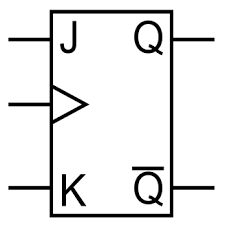
\includegraphics[width=2cm]{ffjk.png}
        \end{figure}
        \begin{solutionorlines}[1in]
            Funciona assim...
        \end{solutionorlines}
        \question Preenchas as lacunas: 
        \begin{parts}
            \part Com relação ao uso de máscaras:
            \begin{subparts}
                \subpart[4] O uso de \fillin[máscaras][3cm] é \fillin[obrigatório][2.5cm] porque \fillin[protege][2cm] todos ao redor.
                \subpart Marque (V) para verdadeiro e (F) para falso.
                \begin{subsubparts}
                    \subsubpart[3] (\fillin[F][0.5cm]) primeira sentença.
                    \subsubpart[3] (\fillin[V][0.5cm]) segunda sentença.
                    \subsubpart[3] (\fillin[F][0.5cm]) terceira sentença.
                    \subsubpart[3] (\fillin[V][0.5cm]) quarta sentença.
                    \subsubpart[3] (\fillin[F][0.5cm]) quinta sentença.
                    \subsubpart[3] (\fillin[V][0.5cm]) sexta sentença.
                    \subsubpart[3] (\fillin[F][0.5cm]) sétima sentença. 
                \end{subsubparts}
            \end{subparts}
        \end{parts}

        \question Questões de múltipla escolha:
        \begin{parts}
            \part[3] Onde vende água?
            \begin{choices}
                \choice Farmácia.
                \choice Mercado.
                \CorrectChoice Mercearia.
                \choice Restaurante.
            \end{choices}

            \part[3] Onde vende água?

            \begin{oneparchoices}
                \choice Farmácia.
                \choice Mercado.
                \CorrectChoice Mercearia.
                \choice Restaurante.
            \end{oneparchoices}

            \part[3] Onde vende água? % Aqui não precisa linha vazia. Começa na outra linha de qualquer forma.
            \begin{checkboxes}
                \choice Farmácia.
                \choice Mercado.
                \CorrectChoice Mercearia.
                \choice Restaurante.
            \end{checkboxes}

            \part[3] Onde vende água? % Sem uma linha vazia, as opções começam na mesma linha
            \begin{oneparcheckboxes}
                \choice Farmácia.
                \choice Mercado.
                \CorrectChoice Mercearia.
                \choice Restaurante.
            \end{oneparcheckboxes}
        \end{parts}
    \end{questions}
\end{document}
% -------------Final do documento-------------